\documentclass[border=8pt]{standalone}
\usepackage{fontspec}
\setmainfont{TeX Gyre Heros}
\setsansfont{TeX Gyre Heros}
\usepackage{tikz}
\usetikzlibrary{arrows.meta,positioning,shapes.geometric,shapes.misc,shapes.symbols,fit,backgrounds,calc,chains}
\definecolor{ink}{HTML}{111827}
\definecolor{band}{HTML}{F3F4F6}
\definecolor{band2}{HTML}{E5E7EB}
\definecolor{accent}{HTML}{1D4ED8}
\definecolor{accentlight}{HTML}{DBEAFE}
\definecolor{warn}{HTML}{B91C1C}
\definecolor{warnlight}{HTML}{FEE2E2}
\definecolor{ok}{HTML}{047857}
\definecolor{oklight}{HTML}{D1FAE5}
\tikzset{
  >={Stealth[length=2.6mm]},
  box/.style={draw=ink, line width=0.6pt, rounded corners=9pt, fill=white, align=center,
              inner sep=4pt, font=\small},
  pill/.style={box, rounded corners=13pt},
  key/.style={box, fill=accentlight, draw=accent, line width=0.9pt},
  soft/.style={box, fill=band},
  dec/.style={draw=ink, line width=0.6pt, diamond, aspect=2.2, align=center, inner sep=1.5pt,
              font=\footnotesize, fill=white},
  arr/.style={->, draw=ink, line width=0.6pt},
  darr/.style={->, draw=ink, line width=0.6pt, dashed},
  lbl/.style={font=\footnotesize, fill=white, inner sep=1.5pt},
  layer/.style={draw=band2, fill=band, rounded corners=6pt},
  title/.style={font=\bfseries\small, align=left, anchor=west},
}
\begin{document}
\sffamily\hyphenpenalty=10000\exhyphenpenalty=10000

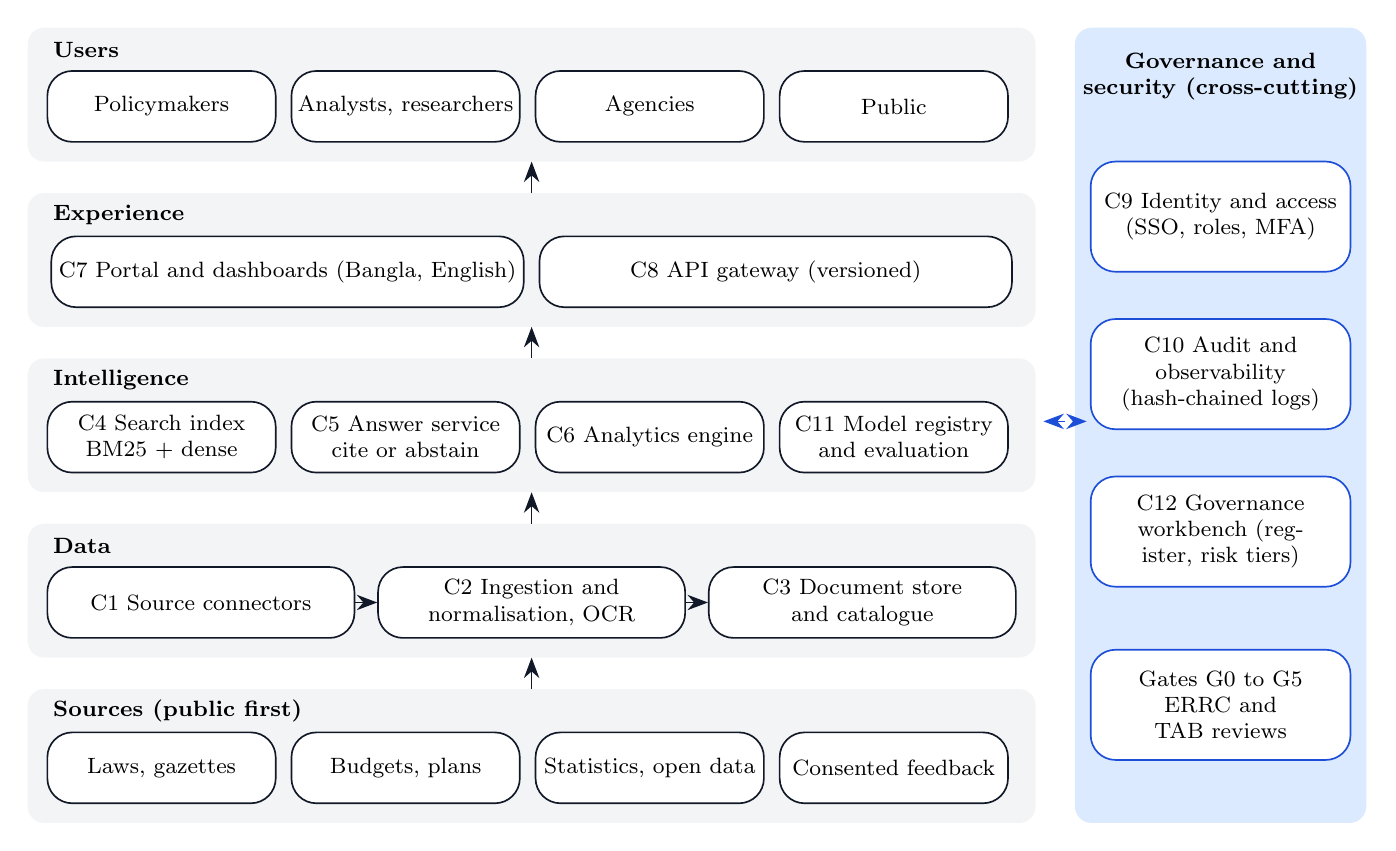
\begin{tikzpicture}
\def\W{128mm}
% layer bands
\foreach \y/\t in {0/Users,-21/Experience,-42/Intelligence,-63/Data,-84/Sources (public first)} {
  \fill[band, rounded corners=6pt] (0,\y mm) rectangle (\W,\y mm-17mm);
  \node[title, font=\bfseries\footnotesize] at (2mm,\y mm-2.8mm) {\t};
}
\tikzset{cell/.style={box, minimum height=9mm, font=\footnotesize, inner sep=2pt}}
% users
\node[cell, minimum width=29mm] at (17mm,-10mm) {Policymakers};
\node[cell, minimum width=29mm] at (48mm,-10mm) {Analysts, researchers};
\node[cell, minimum width=29mm] at (79mm,-10mm) {Agencies};
\node[cell, minimum width=29mm] at (110mm,-10mm) {Public};
% experience
\node[cell, minimum width=60mm] (c7) at (33mm,-31mm) {C7 Portal and dashboards (Bangla, English)};
\node[cell, minimum width=60mm] (c8) at (95mm,-31mm) {C8 API gateway (versioned)};
% intelligence
\node[key, cell, minimum width=29mm] (c4) at (17mm,-52mm) {C4 Search index\\BM25 + dense};
\node[key, cell, minimum width=29mm] (c5) at (48mm,-52mm) {C5 Answer service\\cite or abstain};
\node[cell, minimum width=29mm] (c6) at (79mm,-52mm) {C6 Analytics engine};
\node[cell, minimum width=29mm] (c11) at (110mm,-52mm) {C11 Model registry\\and evaluation};
% data
\node[cell, minimum width=39mm] (c1) at (22mm,-73mm) {C1 Source connectors};
\node[cell, minimum width=39mm] (c2) at (64mm,-73mm) {C2 Ingestion and\\normalisation, OCR};
\node[cell, minimum width=39mm] (c3) at (106mm,-73mm) {C3 Document store\\and catalogue};
% sources
\node[cell, minimum width=29mm] (s1) at (17mm,-94mm) {Laws, gazettes};
\node[cell, minimum width=29mm] (s2) at (48mm,-94mm) {Budgets, plans};
\node[cell, minimum width=29mm] (s3) at (79mm,-94mm) {Statistics, open data};
\node[cell, minimum width=29mm] (s4) at (110mm,-94mm) {Consented feedback};
% flow arrows
\draw[arr] (64mm,-84mm) -- (64mm,-80mm);
\draw[arr] (c1) -- (c2); \draw[arr] (c2) -- (c3);
\draw[arr] (64mm,-63mm) -- (64mm,-59mm);
\draw[arr] (64mm,-42mm) -- (64mm,-38mm);
\draw[arr] (64mm,-21mm) -- (64mm,-17mm);
% governance column
\fill[accentlight, rounded corners=6pt] (\W+5mm,0) rectangle (\W+42mm,-101mm);
\node[title, font=\bfseries\footnotesize, align=center, anchor=north, text width=35mm] at (\W+23.5mm,-2mm) {Governance and security (cross-cutting)};
\tikzset{gcell/.style={box, draw=accent, minimum width=33mm, minimum height=14mm, font=\footnotesize, text width=30mm}}
\node[gcell] at (\W+23.5mm,-24mm) {C9 Identity and access (SSO, roles, MFA)};
\node[gcell] at (\W+23.5mm,-44mm) {C10 Audit and observability (hash-chained logs)};
\node[gcell] at (\W+23.5mm,-64mm) {C12 Governance workbench (register, risk tiers)};
\node[gcell] at (\W+23.5mm,-86mm) {Gates G0 to G5\\ERRC and TAB reviews};
\draw[darr, <->, draw=accent] (\W+1mm,-50mm) -- (\W+6.5mm,-50mm);
\end{tikzpicture}
\end{document}
